\documentclass[10pt]{article}
\usepackage{microtype}
\usepackage{graphicx}
\usepackage{booktabs}
\usepackage{amsmath}
\usepackage{url}
\usepackage{hyperref}
\usepackage{placeins}
\usepackage[accepted]{icml2019}
\usepackage{iftex}
\ifXeTeX
\usepackage{fontspec}
\IfFontExistsTF{Times New Roman}{\setmainfont{Times New Roman}}{\setmainfont{TeX Gyre Termes}}
\fi
\graphicspath{{../results/figures/}}
\icmltitlerunning{Hourly Bikeshare Use with Calendar and Weather Features}
\makeatletter
\renewcommand{\Notice@String}{Machine Learning course project. Individual work.}
\gdef\icmlcorrespondingauthor@text{Yuan Kaige}
\makeatother
\hypersetup{hypertexnames=false,pdftitle={Hourly Capital Bikeshare Use with Calendar and Weather Features},pdfauthor={Yuan Kaige},pdfsubject={Machine Learning course project}}
\newcommand{\NRaw}{12,776,970}
\newcommand{\NTest}{8,758}
\newcommand{\NDev}{8,782}
\newcommand{\NGrid}{17,544}
\newcommand{\NDuplicates}{141}
\newcommand{\NMissingStartStation}{2,700,908}
\newcommand{\NMissingEndStation}{2,797,787}
\newcommand{\NNegativeDuration}{371}
\newcommand{\NLongDuration}{9,686}
\newcommand{\NShortDuration}{264,913}
\newcommand{\NOutsideMonth}{1,602}
\newcommand{\NAmbiguous}{1,227}
\newcommand{\NAmbiguousTwentyFour}{645}
\newcommand{\NAmbiguousTwentyFive}{582}
\newcommand{\NAssigned}{12,775,602}
\newcommand{\NAnnualTwentyFour}{6,113,573}
\newcommand{\NAnnualTwentyFive}{6,662,029}
\newcommand{\AnnualGrowth}{8.97}
\newcommand{\NValidation}{4,415}
\newcommand{\PythonVersion}{3.14.6}
\newcommand{\SklearnVersion}{1.9.0}
\newcommand{\PrimaryMAE}{166.43}
\newcommand{\PrimaryRMSE}{241.86}
\newcommand{\PrimaryRSquared}{0.855}
\newcommand{\PrimaryBias}{-67.50}
\newcommand{\PrimaryValRMSE}{220.09}
\newcommand{\BoostTimeRMSE}{288.48}
\newcommand{\BaselineRMSE}{347.01}
\newcommand{\WeatherRMSEGain}{16.16}
\newcommand{\BaselineRMSEGain}{30.30}
\newcommand{\WeatherMAEChange}{24.30}
\newcommand{\BootstrapLow}{16.49}
\newcommand{\BootstrapHigh}{32.42}
\newcommand{\WorstHour}{2025-03-29 at 16:00 local time}
\newcommand{\WorstObserved}{2,930}
\newcommand{\WorstPredicted}{1,581.55}
\newcommand{\PeakMAE}{273.52}
\newcommand{\OtherMAE}{143.11}
\newcommand{\WetMAE}{193.54}
\newcommand{\DryMAE}{161.45}
\newcommand{\HotMAE}{257.05}
\newcommand{\ColdMAE}{102.51}

\begin{document}
\twocolumn[
\icmltitle{Hourly Capital Bikeshare Use with Calendar and Weather Features: \\ A Study of Official 2024--2025 Trip Records}
\begin{icmlauthorlist}
\icmlauthor{Yuan Kaige}{course}
\end{icmlauthorlist}
\icmlaffiliation{course}{Machine Learning; student ID 202612231033; individual project}
\vskip 0.3in
]
\printAffiliationsAndNotice{}

\begin{abstract}
This project studies hourly recorded departures in the Capital Bikeshare system using all 24 monthly files from 2024 and 2025. Exploratory analysis describes calendar and weather patterns, while regression compares a weekday--hour mean baseline, Ridge, random forest and histogram gradient boosting. Model settings are selected using expanding time windows within 2024, with 2025 reserved for final testing. On \NTest\ eligible test hours, the validation-selected gradient boosting model with calendar and ERA5 weather features obtains MAE \PrimaryMAE\ and RMSE \PrimaryRMSE\ rides per hour, compared with RMSE \BoostTimeRMSE\ for its calendar-only version. Weather improves this model's test RMSE by \WeatherRMSEGain\%, but errors remain larger at weekday peaks and in hot or wet conditions. The target measures recorded departures rather than unmet demand, and retrospective weather supports estimation conditional on known conditions rather than a verified advance forecasting service.
\end{abstract}

\section{Introduction}
Public bicycle systems provide an alternative for short urban trips. Operators need to understand when riders use the service because busy periods can place pressure on bicycles, docks and staff. The relevant patterns vary within a day, across the week and across seasons. Weather may add information beyond these regular patterns. For example, two otherwise similar weekday afternoons can have different riding conditions. This makes bikeshare use a useful setting for studying both exploratory data analysis and regression.

The project focuses on Capital Bikeshare and uses its official trip releases for 2024 and 2025 \citep{capitaldata}. It does not substitute the familiar older public bikeshare benchmark. The target is the number of recorded trip starts across the whole published system in an hourly interval. This choice makes a manageable modelling table from millions of trips and avoids requiring station-level forecasts for hundreds of locations. It also has a clear limitation: recorded starts reflect both willingness to ride and whether a usable bicycle was available. Someone who could not find a bicycle generates no departure record. Therefore, the term demand in the project topic is interpreted as observed use, not the full underlying demand.

Three questions guide the analysis. First, how does hourly use vary with time of day, weekdays, weekends and season? Second, does adding weather improve prediction compared with calendar features alone? Third, how do standard regression families compare, and which time or weather groups have larger errors? The project answers these questions using the same audited target and a common chronological evaluation design.

The main comparison is deliberately modest. It uses methods available in scikit-learn and a small parameter grid, rather than a large search or a deep learning system. A simple baseline shows how much can be predicted from the weekly cycle alone. Ridge tests an additive relationship, and two tree ensembles allow nonlinear relationships and interactions. The weather comparison is repeated within each model family so that a change in model family is not mistaken for a benefit from weather.

All modelling decisions are made using 2024. The whole of 2025 is then evaluated without retuning. This is more relevant to transfer into a later year than a random split of individual hours. Source code, the executed notebook, a derived hourly table and acquisition instructions accompany the study. The project repository is \url{https://github.com/Yuan-KG/Project_BikeSharing}.

\section{Related Work}
Weather and bikeshare use have been studied in the same region. \citet{gebhart2014weather} linked hourly Washington, DC bikeshare activity to weather and reported associations with conditions including rain, cold and humidity. This supports examining weather as a candidate source of predictive information. The earlier study describes another period and modelling setting, so its estimates are not treated as effects that must hold in the present records. Its publisher abstract and bibliographic record inform this discussion; no unavailable full-text result is reproduced here.

\citet{torres2024forecasting} compared machine learning approaches including random forest, gradient boosting and neural networks for a New York bikeshare application. That work provides a reason to compare more than one regression family. Its spatial target, operational context and feature availability differ from the present system-wide hourly count. Numerical results from that application would therefore not be a fair benchmark for this project.

\citet{fanaee2014event} used bike-sharing usage data in research on event labelling. That is useful background for the widely used older Capital Bikeshare dataset, but it is not evidence that a particular regression model will be best here. This project instead downloads the provider's new monthly records and preserves the complete 2025 year as a later test period. The contribution is a reproducible course-scale comparison with explicit audit, time alignment and weather ablation, rather than a claim of a new algorithm.

Weather itself also requires a methodological distinction. ERA5 is a retrospective global reanalysis that combines observations with a numerical model \citep{hersbach2020era5}. Open-Meteo supplies a convenient historical interface \citep{zippenfenig2023openmeteo,openmeteo}. Neither the use of a historical endpoint nor strong test accuracy proves that equally accurate weather would have been available before each predicted hour. This distinction determines the scope of the conclusions.

\section{Data and Preprocessing}
\subsection{Sources and scope}
The official S3 listing contains all 24 requested monthly ZIP files, from January 2024 through December 2025. The local raw collection contains \NRaw\ rows. Each file is downloaded from the provider's public download service, checked against its listed byte size, checked with ZIP member CRCs and assigned a SHA-256 hash. The manifest records file names, full source URLs, UTC retrieval timestamps, S3 modification times and archive members. Downloading took place on 13 November 2026. Raw archives remain unchanged.

All releases have the same 13-column schema: ride ID, bicycle type, start and end timestamps, start and end station names and IDs, start and end coordinates, and member/casual type. Timestamp precision changes from seconds to milliseconds in later records, so parsing supports both representations. Files are read in chunks of 200,000 rows. A disk-backed SQLite index tracks previously observed ride IDs across chunks and files. This avoids keeping the entire trip table in memory.

The project uses the provider's released scope. It does not add GPS-based geographical exclusions or select particular stations. Such exclusions would change the meaning of system-wide use and require additional justifications. Station, bicycle type and membership fields are audited but never used as hourly prediction inputs, because their same-hour totals could reveal parts of the target.

\subsection{Identity, missingness and time checks}
There are \NDuplicates\ repeated ride-ID rows. All have conflicting row contents rather than identical full records. The first occurrence is retained under the rule fixed before modelling. Without an independent transaction log, it is not possible to determine whether every conflict is a corrected record or a reused identifier. The number is small relative to the full collection, but the rule and its limitation remain explicit.

There are no unparseable start or end timestamps and no missing ride IDs. Missing optional fields occur in station and coordinate information, including \NMissingStartStation\ missing start-station IDs and \NMissingEndStation\ missing end-station IDs in the raw rows. These fields are not required to count a valid departure, so their absence does not cause a row to be dropped. The full field-by-month missingness table is saved in the audit and shown in the notebook.

End times are checked for plausibility. Among retained identity records, \NNegativeDuration\ local-clock durations are negative, \NLongDuration\ exceed 24 hours, and \NShortDuration\ are between zero and 60 seconds. These categories are diagnostics, not extra exclusion rules. The target is a start count; removing a valid start because of an unusual end would impose another definition of use. Local-clock differences around daylight saving transitions also require care and are not equivalent to elapsed UTC duration.

The provider's descriptive webpage says that short trips are filtered upstream \citep{capitaldata}. The modern files nevertheless contain the short durations listed above. The analysis reports what is actually present rather than claiming that the older webpage description exactly matches these releases. Likewise, \NOutsideMonth\ rows begin outside the month named in their ZIP. Their valid starts fall within the overall study window and are assigned to their true calendar hour after cross-file identity checks. Thus, file month and start month are not assumed to be interchangeable.

\begin{table}[t]
\caption{Row accounting. End-time diagnostics do not remove a valid start. The unresolved DST rows are retained separately.}
\label{tab:audit}
\centering
\begin{tabular}{lr}
\toprule
Stage & Rows \\
\midrule
Raw monthly rows & 12,776,970 \\
Repeated IDs removed & 141 \\
Invalid or out-of-scope starts & 0 \\
Unresolved DST starts & 1,227 \\
Assigned hourly departures & 12,775,602 \\
\bottomrule
\end{tabular}

\end{table}

\subsection{Time zone and daylight saving}
Trip timestamps have no per-record UTC offset. They are interpreted as local wall time in America/New\_York. This is an explicit source assumption. Calendar features use that local zone, while aggregation and weather joins use a unique UTC hourly index. The grid includes the 2024 leap day and contains \NGrid\ actual hours across the two local calendar years.

At the autumn clock change, the local 01:00 hour occurs twice. The files do not provide enough information to assign each naive start to a unique occurrence. There are \NAmbiguous\ such starts in total: \NAmbiguousTwentyFour\ in 2024 and \NAmbiguousTwentyFive\ in 2025. Their combined local-hour counts are preserved in a separate table. Both candidate UTC target hours each year are marked missing and excluded from modelling. This removes four hours from the two-year evaluation grid without pretending that missing counts are zero. No starts fall in a nonexistent spring-forward local hour.

Every expected local date has recorded trips, all requested monthly archives pass integrity checks, and every non-ambiguous hourly bin contains at least one trip. There are therefore no zero-hour bins to fill in the final collection. This observation follows the coverage checks; it is not produced by replacing all missing values with zeros. It cannot prove that every source record was captured or that no partial upstream outage occurred. The final eligible table has \NDev\ development hours and \NTest\ test hours, with \NAssigned\ assigned departures overall.

\subsection{Weather acquisition and interval alignment}
The weather request explicitly selects ERA5 rather than Open-Meteo's changing default combination \citep{openmeteo}. The requested Washington coordinate is 38.9072 N, 77.0369 W. The response identifies a grid location of 39.0 N, 77.0 W and elevation 25 m. ERA5's atmospheric grid is about 0.25 degrees, so this is a regional weather representation rather than an observation at every bikeshare station \citep{copernicus}.

Five variables are used: 2 m temperature in degrees Celsius, 2 m relative humidity in percent, precipitation in millimetres, total cloud cover in percent and 10 m wind speed in kilometres per hour. The raw JSON and metadata preserve the exact API URL, request parameters, units, model and retrieval time. The requested UTC date range extends from 1 January 2024 through 2 January 2026 so that the local study boundaries and the final rainfall interval are covered. Weather values are complete on every modelling hour.

The join respects the meaning of each variable. For a departure target in $[t,t+1\mathrm{h})$, temperature, humidity, cloud and wind use the timestamp at $t$. The API's precipitation value at $t+1\mathrm{h}$ is the cumulative precipitation over the preceding hour, so it describes that target interval \citep{openmeteo}. UTC Unix timestamps are used to avoid the API's fixed-offset ISO behaviour across DST changes. Same-interval precipitation is intentionally retrospective information. This is a comparison under known weather, not a claim about an operational forecast available at $t$.

Trip records are used under the Capital Bikeshare Data License Agreement \citep{capitallicense}. Original ZIPs are kept locally, and the repository provides official acquisition instructions rather than an independent raw-data mirror. Its small derived table is source material for this non-commercial study. Weather data are attributed to Open-Meteo and ERA5/Copernicus under CC BY 4.0, with variable selection and interval alignment documented \citep{openmeteolicense}.

\section{Exploratory Data Analysis}
The development EDA uses 2024. The two-year monthly comparison is produced after model selection is fixed and serves as a descriptive test-period comparison. Counts below exclude unresolved DST starts, whose totals remain available separately. This distinction matters when comparing published annual totals with the exact modelling target.

\subsection{Calendar patterns}
Figure~\ref{fig:monthly} shows strong within-year variation. There are \NAnnualTwentyFour\ eligible departures in 2024 and \NAnnualTwentyFive\ in 2025, an increase of \AnnualGrowth\%. However, growth is not uniform across the calendar. The largest monthly count in 2024 is in October, whereas the corresponding 2025 month is July. A single annual growth factor would therefore hide important changes. The comparison alone does not identify their causes.

\begin{figure*}[!tbp]
\centering
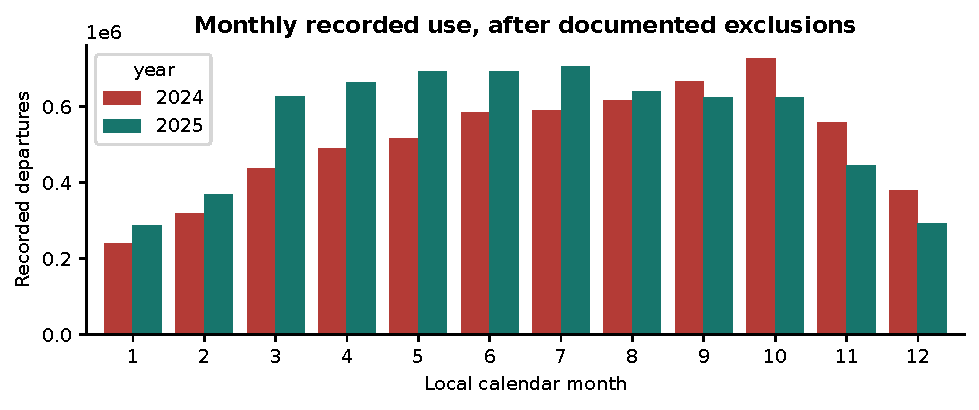
\includegraphics[width=\textwidth]{monthly_counts.pdf}
\caption{Monthly departures assigned to their actual start month after the documented exclusions. Both years use the same processing rule. This is a post-selection descriptive comparison, not an additional tuning target.}
\label{fig:monthly}
\end{figure*}

Figure~\ref{fig:profiles} compares the 2024 mean daily profiles. Weekdays show a morning rise and a stronger late-afternoon peak. Weekend use is concentrated more broadly in the afternoon. These shapes support using hour and weekday together rather than fitting one daily pattern for every day. The weekday--hour mean baseline directly captures this joint weekly profile. Nevertheless, averaging all weeks together cannot respond to a particular rainy day or to seasonal differences.

These are system-wide patterns. A commuter station and a leisure destination can have different profiles even if their totals contribute to the same curve. The analysis cannot infer that every station has the average peak or that every weekday ride is a commute. It also uses a calendar weekday indicator, not a direct observation of each rider's work schedule. Federal holidays are represented separately in modelling but do not cover every school break or local event.

\begin{figure*}[!tbp]
\centering
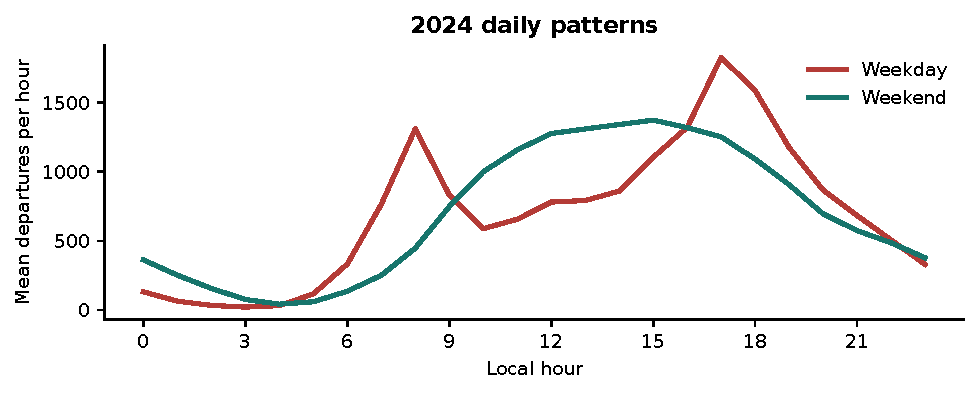
\includegraphics[width=\textwidth]{hour_profiles.pdf}
\caption{Mean 2024 hourly departures on weekdays and weekends. Averages exclude the two unresolved fall-back target hours. The curves describe observed use and do not classify individual trip purposes.}
\label{fig:profiles}
\end{figure*}

\subsection{Weather associations}
Figure~\ref{fig:weather} groups 2024 hours by temperature and whether interval precipitation is positive. Use generally rises from colder bins towards warmer bins, and wet and dry groups often differ. These are unadjusted averages. Temperature, sunlight, season and hour are correlated, and the distribution of rainy hours is not identical to that of dry hours. The plot motivates a predictive comparison but does not estimate the causal effect of increasing temperature or removing rain.

Bin sizes are supplied in the notebook because the extreme temperature groups contain fewer hours. The regression experiment uses continuous weather values rather than these coarse bins. The wet/dry label is used later for error diagnosis; it is not an additional feature extracted from the trip target. In particular, no membership counts, bicycle-type counts or same-hour station activity are introduced through the EDA.

\begin{figure*}[!tbp]
\centering
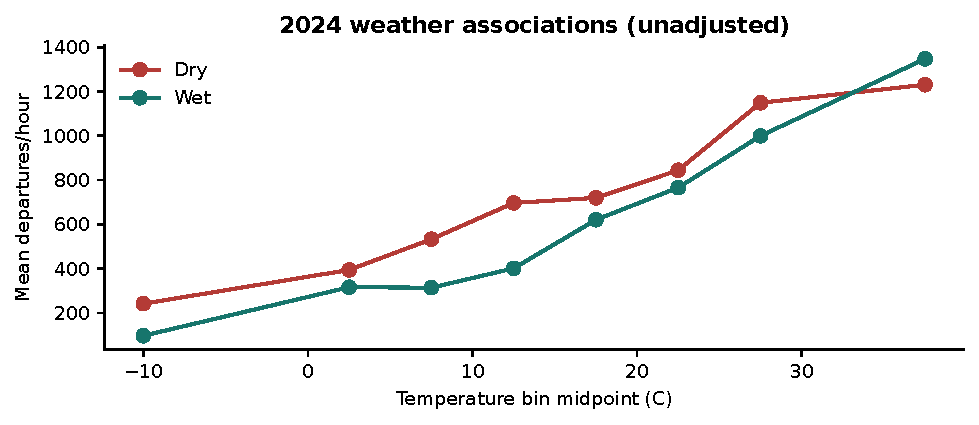
\includegraphics[width=\textwidth]{weather_associations.pdf}
\caption{Unadjusted 2024 departures by temperature bin midpoint and interval precipitation. Wet means precipitation greater than zero. Unequal season and time distributions prevent a causal reading of these averages. Weather data: Open-Meteo, ERA5/Copernicus (CC BY 4.0), aligned as described in Section 3.}
\label{fig:weather}
\end{figure*}

\section{Methods and Experimental Setup}
\subsection{Chronological development and testing}
The full 2025 year is the final test set. Development uses three expanding windows: January--June 2024 training with July--August validation; January--August training with September--October validation; and January--October training with November--December validation. Boundaries follow local dates. The three validation windows together contain \NValidation\ eligible hours. Each fold uses only earlier labels to fit both its model and preprocessing.

Candidate settings are ranked by RMSE pooled over the validation predictions. Pooling gives each eligible hour equal weight rather than each differently sized window equal weight. One setting is selected for each family and feature set. The primary model is the candidate with the lowest validation RMSE across those selected regressors. Its identity and all six settings are written to a selection file before any 2025 prediction or score is calculated. All six settings are then refitted on the complete eligible 2024 data and evaluated on the same \NTest\ test hours.

An expanding-window design avoids using future training records to predict earlier validation hours, but it is not a perfect simulation of every future year. In particular, the earliest training window does not contain a complete annual cycle. A month indicator unseen in a fold is ignored by the one-hot encoder, while the cyclic calendar terms still provide a seasonal representation. This can make the first validation period difficult. Final fitting includes all months of 2024. There is no random train/test split and no adjustment after inspecting the final test errors.

\subsection{Features and preprocessing}
The calendar-only set contains hour, weekday, month, weekend, a U.S. federal-holiday indicator, a weekday--hour interaction, and sine/cosine pairs for hour and day of year. The hourly cycle uses period 24; the annual pair uses 365.2425 days. The continuous encoding makes adjacent cycle values close, including across midnight or the year boundary. Month remains available as a coarse seasonal effect. The weekday--hour feature lets a linear model represent a different hourly pattern for each weekday.

For Ridge, hour, weekday, month and weekday--hour are one-hot encoded. Other calendar values and any weather variables are standardized. Imputation, scaling and category discovery are fitted inside each training pipeline. Unknown validation categories are handled without inspecting the validation distribution. For the tree models, the fixed numeric feature set is median-imputed using training data. Their split rules need no standardization. The hourly table contains no weather gaps, but the imputation policy remains part of the reproducible pipeline.

The second feature set adds the five weather measurements to the identical calendar set. Year, an extrapolating trend, target lags and rolling target averages are omitted. This keeps the question focused on calendar versus known weather and allows every test hour to be estimated without feeding observed 2025 ride counts back into the model. A future operational system could use lagged information available at prediction time, but that is a different experiment. Station counts and trip-end fields are never used as predictors.

\subsection{Models and parameter choices}
The baseline estimates the training mean count for each weekday and hour. A training global mean is the fallback for an unseen combination. This provides an understandable reference: it predicts a typical Monday at 08:00 from earlier Mondays at 08:00. It cannot distinguish a winter Monday from a summer Monday or react to weather.

Ridge minimizes squared error with an $L_2$ coefficient penalty. The candidate penalty values are 1, 10 and 100. An SVD solver is used for numerical stability when the encoded calendar columns are correlated. The linear model is an additive prediction rule, but it does not automatically represent temperature-by-hour or weather-by-season interactions.

Random forest averages 160 regression trees. The candidate minimum leaf sizes are 2 and 8, while other settings use scikit-learn defaults. Histogram gradient boosting adds trees sequentially to reduce squared error. It uses 250 iterations, learning rate 0.06 and $L_2$ regularization 1, with 15 or 31 maximum leaves per tree as candidates. Internal early stopping is disabled so there is no random internal validation partition. The random seed is 42, and thread use is limited to four. The chosen settings are listed in Table~\ref{tab:settings}.

\begin{table}[t]
\caption{Settings selected using 2024 only. RF has 160 trees. Boosting uses 250 iterations, learning rate 0.06 and regularization 1.}
\label{tab:settings}
\centering
\begin{tabular}{lll}
\toprule
Model & Inputs & Selected setting \\
\midrule
Ridge & Time & alpha=1 \\
Ridge & + weather & alpha=10 \\
Random forest & Time & leaf min=2 \\
Random forest & + weather & leaf min=2 \\
Gradient boosting & Time & leaves=31 \\
Gradient boosting & + weather & leaves=15 \\
\bottomrule
\end{tabular}

\end{table}

All families are evaluated with predictions clipped below at zero. This common rule is fixed before validation because a negative departure count is not meaningful. Predictions remain continuous estimates rather than being rounded to an integer. The limited grid is intended for an ordinary computer, and it does not establish that these are the best possible versions of each model family. The final environment uses Python \PythonVersion\ and scikit-learn \SklearnVersion.

\subsection{Metrics and diagnostic groups}
For $n$ evaluated hours, observed counts $y_i$ and estimates $\hat{y}_i$, the two main errors are
\begin{equation}
\mathrm{MAE}=\frac{1}{n}\sum_{i=1}^{n}|\hat{y}_i-y_i|,
\end{equation}
\begin{equation}
\mathrm{RMSE}=\sqrt{\frac{1}{n}\sum_{i=1}^{n}(\hat{y}_i-y_i)^2}.
\end{equation}
Both are measured in rides per hour. RMSE gives more weight to large misses, which is useful when busy hours are difficult. $R^2$ is also reported against variation in the test observations. Signed mean error is the average of estimate minus observation, so a negative value means underestimation. A good overall score does not guarantee small errors in every group.

The pre-specified peak group consists of weekdays at 07:00--09:59 and 16:00--18:59. Other comparisons cover weekdays versus weekends, dry versus positive-precipitation hours, and temperatures below 5 C, from 5 to 25 C, and above 25 C. These groups overlap and are not causal strata. Counts and mean observed use accompany their errors. A paired day bootstrap with 2,000 resamples and seed 42 provides descriptive 95\% intervals for the MAE improvement from weather within each family. Resampling days preserves within-day pairing, but does not capture every form of long-term dependence or future change.

\section{Results and Discussion}
\subsection{Validation and model comparison}
Table~\ref{tab:results} reports selected-candidate validation RMSE and the final test metrics. The primary model is the weather-augmented histogram gradient boosting regressor with 15 leaves. Its 2024 validation RMSE is \PrimaryValRMSE. Selection therefore favours it before the 2025 results are examined. The baseline's validation result is reported for context, while the same fixed weekly-mean rule is used at test time.

\begin{table*}[!tbp]
\caption{Selected settings and final evaluation. Every test row uses the same \NTest\ eligible 2025 hours. Validation RMSE pools the three 2024 windows. Errors and bias are rides per hour. The primary model is chosen by 2024 validation, not by this test table.}
\label{tab:results}
\centering
\begin{tabular}{llrrrrr}
\toprule
Model & Inputs & Val. RMSE & Test MAE & Test RMSE & $R^2$ & Bias \\
\midrule
Weekday--hour mean & Time & 358.48 & 240.98 & 347.01 & 0.702 & -64.40 \\
Ridge & Time & 329.86 & 216.32 & 307.07 & 0.767 & -50.78 \\
Ridge & Time + weather & 342.04 & 201.83 & 284.63 & 0.800 & -63.42 \\
Random forest & Time & 306.26 & 188.54 & 290.81 & 0.791 & -63.17 \\
Random forest & Time + weather & 243.84 & 168.79 & 250.80 & 0.844 & -66.92 \\
Gradient boosting & Time & 322.55 & 190.73 & 288.48 & 0.794 & -62.45 \\
Gradient boosting & Time + weather & 220.09 & 166.43 & 241.86 & 0.855 & -67.50 \\
\bottomrule
\end{tabular}

\end{table*}

The simple baseline reaches test RMSE \BaselineRMSE, showing that the weekly cycle already explains a substantial part of observed use. Calendar-only Ridge and tree models improve on that reference, but errors remain sizeable. The primary model reaches MAE \PrimaryMAE, RMSE \PrimaryRMSE\ and $R^2=\PrimaryRSquared$. Relative to the baseline, its RMSE is lower by \BaselineRMSEGain\%. This is a comparison on one later year, not a guarantee of the same reduction elsewhere.

\begin{figure*}[!tbp]
\centering
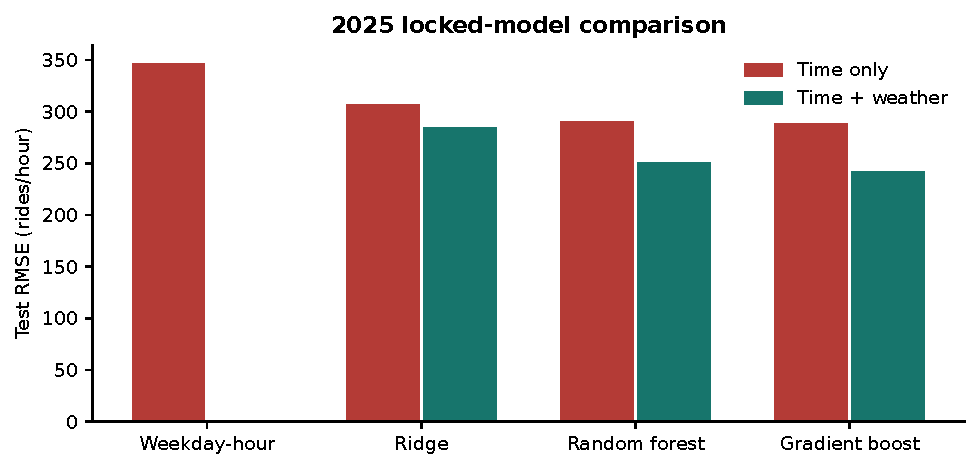
\includegraphics[width=\textwidth]{test_comparison.pdf}
\caption{Test RMSE for the fixed model settings. Weather is compared within each regression family; the baseline has only a calendar version. All predictions are non-negative and use identical target hours.}
\label{fig:comparison}
\end{figure*}

The tree models can partition the relationship by both weather and calendar conditions. Their lower errors are consistent with interactions that an additive Ridge model cannot represent directly. This is a reasonable explanation for the model comparison, rather than proof about the true mechanism. Model complexity, feature encoding and the small parameter grid all differ. The experiment does not isolate each of those design choices separately.

\subsection{What does weather add?}
For histogram gradient boosting, adding weather changes RMSE from \BoostTimeRMSE\ to \PrimaryRMSE, a \WeatherRMSEGain\% reduction, and reduces MAE by \WeatherMAEChange\ rides per hour. Random forest and Ridge also improve on their own calendar-only test versions. Figure~\ref{fig:comparison} makes these within-family comparisons visible. The result answers the second research question for this target, period and evaluation setup.

Validation is more nuanced. Adding weather improves the selected tree candidates, while the selected weather Ridge candidate has worse pooled validation RMSE than calendar-only Ridge. Weather is therefore not uniformly beneficial for every algorithm and development period. The 2025 Ridge improvement does not justify changing its setting after testing. This difference also warns against selecting an approach from a single favourable final score.

The paired day bootstrap gives a primary-model MAE improvement of \WeatherMAEChange\ rides per hour, with a descriptive 95\% interval of [\BootstrapLow, \BootstrapHigh]. This summarizes paired error differences across the observed test days. It is not a causal weather effect or an interval for all future years. The experiment changes the information supplied to a prediction model; it does not randomly change real weather while holding travel conditions fixed.

\subsection{When are errors larger?}
Table~\ref{tab:groups} reports the pre-specified primary-model groups. Peak weekday hours have MAE \PeakMAE\ compared with \OtherMAE\ in other hours. Their mean count is also much higher. Larger absolute errors during busy periods therefore do not, by themselves, show a larger percentage error. Weekday and weekend overall MAEs are similar even though their hourly shapes differ. This suggests that the time features capture much of the average profile difference, while individual busy hours remain challenging.

\begin{table*}[!tbp]
\caption{Primary-model test errors by pre-specified groups. Categories overlap. Temperature and wet/dry groups describe the aligned ERA5 input, not station-specific conditions. Positive bias indicates overestimation.}
\label{tab:groups}
\centering
\begin{tabular}{lrrrrr}
\toprule
Group & Hours & Mean count & MAE & RMSE & Bias \\
\midrule
All & 8,758 & 760.68 & 166.43 & 241.86 & -67.50 \\
Weekday & 6,264 & 759.81 & 167.07 & 242.97 & -69.96 \\
Weekend & 2,494 & 762.85 & 164.81 & 239.06 & -61.30 \\
Peak weekday & 1,566 & 1386.34 & 273.52 & 350.86 & -140.16 \\
Other hours & 7,192 & 624.45 & 143.11 & 210.79 & -51.68 \\
Dry & 7,400 & 769.90 & 161.45 & 233.92 & -64.51 \\
Wet & 1,358 & 710.46 & 193.54 & 281.24 & -83.77 \\
Cold $<5$ C & 1,978 & 359.15 & 102.51 & 152.16 & -15.71 \\
Mild 5--25 C & 5,446 & 763.10 & 167.44 & 240.72 & -56.61 \\
Hot $>25$ C & 1,334 & 1346.16 & 257.05 & 336.40 & -188.73 \\
\bottomrule
\end{tabular}

\end{table*}

Wet hours have MAE \WetMAE\ compared with \DryMAE\ for dry hours. Hot hours above 25 C have MAE \HotMAE, while cold hours below 5 C have MAE \ColdMAE. Cold-hour counts are lower on average, so the smaller absolute error is not evidence that winter behaviour is fully understood. Wet is defined by any positive modelled precipitation; it groups light rain with heavier precipitation and can miss local spatial differences. These operational definitions matter when interpreting error groups.

\begin{figure*}[!tbp]
\centering
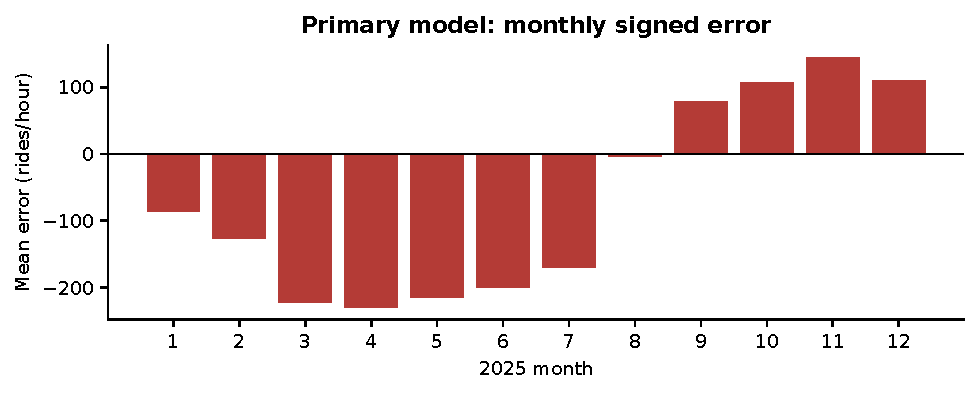
\includegraphics[width=\textwidth]{monthly_bias.pdf}
\caption{Primary-model mean signed error by 2025 month. A changing sign shows why one overall bias value is insufficient. No correction is fitted to these test-period errors.}
\label{fig:bias}
\end{figure*}

The overall signed error is \PrimaryBias\ rides per hour. However, Figure~\ref{fig:bias} shows that this bias is not constant: the model underestimates strongly in much of the first half of 2025 and overestimates in the final months. August has a comparatively small signed bias. Annual growth alone therefore does not explain the error pattern. A single upward adjustment could improve some months and worsen others; no such correction is selected from the test observations. Additional observed-versus-estimated and hourly-bias plots are available in the notebook.

The largest absolute error occurs at \WorstHour, when \WorstObserved\ departures are recorded and the estimate is \WorstPredicted. Several large misses occur in late March. A local event, tourism, changing system availability or a different weather-use relationship could contribute, but none is verified by this dataset. Assigning a named event as the cause without independent evidence would overstate the result. The notebook provides the actual timestamps and inputs so that such cases can be investigated later.

The monthly audit also shows that the number of distinct station IDs with observed starts changes from 758 in January 2024 to 815 in December 2025. This is evidence that the active recorded footprint differs, but it is not a direct inventory of installed stations. ID changes, temporary inactivity and coverage can affect it. System growth is one plausible source of distribution shift, alongside travel behaviour and exceptional conditions. The present models have no direct system-capacity input, so their calendar and weather relationships can become outdated.

\FloatBarrier
\section{Limitations}
\textbf{Observed use and aggregation.} The target counts published starts and cannot reveal riders turned away by empty stations, unusable bicycles or service restrictions. System-wide aggregation can also hide local shortages and opposite station flows. Good aggregate accuracy is not enough to plan rebalancing at a particular station. A capacity-aware station study would need additional data, availability checks and a different evaluation target.

\textbf{Weather availability and representativeness.} One ERA5 grid location is a coarse representation for a system spread over the Washington region. Local showers, wind exposure and urban conditions can differ. Reanalysis uses retrospective information, including same-interval precipitation. An advance forecast application would need archived forecasts with known issue times and horizons, plus a fresh evaluation. The current weather benefit should not be advertised as the verified benefit of a live forecast API.

\textbf{Source uncertainty.} CRC and hash checks show that the downloaded files are intact, not that the provider captured every trip. The records contain conflicting IDs, unexpected durations and starts outside release months. Boundary starts released in archives outside the requested 24-file collection could also be absent. Annual counts therefore describe this downloaded collection rather than a guaranteed complete transaction census. Fall-back hours remain unresolved rather than being assigned by guesswork.

\textbf{Change over time.} Only one development year and one test year are observed. The station footprint, bicycle mix, prices, promotions, rider composition and travel patterns may change. Most of these variables are absent from the feature set. The pronounced monthly bias reversal illustrates that relationships can change even within one year. Regular updating might help, but that would need rolling deployment experiments rather than fitting a correction to this final test set.

\textbf{Comparison scope.} The parameter search is limited, and there is no claim of global model optimality. A count-based loss, station features, valid lagged counts or a richer calendar could be worth testing in a new pre-specified study. The bootstrap interval summarizes this particular year and is not a full uncertainty model. Feature associations, model ranking and potential feature importance would all remain predictive evidence rather than causal conclusions.

\section{Conclusion}
The project combines an audit of \NRaw\ official trip rows with exploratory analysis and a chronological regression comparison. The records show clear daily, weekly and seasonal patterns, but the later year does not follow a uniform growth pattern. Known historical weather improves the primary model's 2025 RMSE by \WeatherRMSEGain\% relative to its calendar-only version. Histogram gradient boosting selected on 2024 obtains MAE \PrimaryMAE\ and RMSE \PrimaryRMSE\ rides per hour on 2025. Busy weekday hours, wet conditions and hot periods retain larger absolute errors, and monthly bias changes sign. These results support weather-aware estimation of recorded use while leaving unmet demand, operational forecast availability and future system changes as important open limits.

\bibliography{references}
\bibliographystyle{icml2019}
\end{document}
